\documentclass[a4paper,11pt]{article}
% --- Encoding and language ---
\usepackage[utf8]{inputenc}
\usepackage[english]{babel}
% ne pas charger de package math → LaTeX garde CM pour les maths
\usepackage{microtype}
\usepackage{xspace}
\usepackage{setspace}
% --- Page layout ---
\usepackage{geometry}
\geometry{
  a4paper,
  total={170mm,257mm},
  left=20mm,
  right=20mm,
  top=20mm,
  bottom=20mm
}
\setlength{\headheight}{14pt}
% --- Section and title formatting ---
\usepackage{titlesec}
\setcounter{tocdepth}{2}
\titleformat{\section}[hang]{\normalfont\Large\bfseries}{\thesection}{1em}{}
\titleformat{\subsection}[hang]{\normalfont\large\bfseries}{\thesubsection}{1em}{}
\titleformat{\subsubsection}[hang]{\normalfont\normalsize\bfseries}{\thesubsubsection}{1em}{}
\newcommand{\subsubsubsection}[1]{\paragraph{#1}\mbox{}\\}
% --- Mathematics and symbols ---
\usepackage{amsmath, amsfonts, amssymb, mathrsfs, stmaryrd}
\usepackage{siunitx}
% --- Typography ---
\usepackage{newpxtext, newpxmath}
% --- Graphics and figures ---
\usepackage{graphicx, subcaption, float, wrapfig}
\usepackage[tikz]{bclogo}
\usepackage{sidecap}
% --- Tables ---
\usepackage{booktabs}                          % <-- added
\usepackage{multirow, array, makecell}
% --- Paragraphs ---
\usepackage{ragged2e}
\setlength{\parindent}{0pt}
\newcommand{\myindent}{\hspace*{1.5em}}
% --- List management ---
\usepackage{enumitem}
% --- References and hyperlinks ---
\usepackage{url, hyperref}
\usepackage{cleveref}                          % <-- added (must be after hyperref)
% --- Glossary ---
%\usepackage{glossaries, glossaries-extra}
%\makeglossaries
%\input{glossary}
% --- Headers and footers ---
\usepackage{fancyhdr}
\pagestyle{fancy}
\fancyhf{}
\renewcommand\headrulewidth{1pt}
\fancyhead[R]{\nouppercase{\leftmark}}
\fancyhead[L]{Master 2 Internship report}
\fancyfoot[C]{\thepage}
% --- Miscellaneous tools ---
\usepackage[ruled,vlined]{algorithm2e}
\usepackage{lettrine}
\usepackage{pifont}
\usepackage{pdfpages}
\usepackage{eurosym}
\usepackage{listings}
\usepackage{changepage}
\usepackage[normalem]{ulem}
\usepackage{frcursive}
\usepackage{fvextra}
\usepackage{comment}
\usepackage{tikz}
\usepackage{import}
\usepackage[numbers,sort&compress]{natbib}
\usepackage{placeins}
% --- Macros : annotations ---
\newcommand{\noteBastien}[1]{\textcolor{blue}{#1}}
\newcommand{\noteMichele}[1]{\textcolor{red}{#1}}
\newcommand{\noteDavid}[1]{\textcolor{green}{#1}}
% --- Macros : code identifiers ---
\newcommand{\UnsignedInt}{\texttt{UnsignedInt}\xspace}
\newcommand{\UnsignedInts}{\texttt{UnsignedInts}\xspace}
\newcommand{\BitSet}{\texttt{BitSet}\xspace}
\newcommand{\BitSets}{\texttt{BitSets}\xspace}
\newcommand{\Bits}{\texttt{Bits}\xspace}
% --- Additional customisation ---
\addto\captionsfrench{\renewcommand{\contentsname}{\center{Table des matières}}}
\renewcommand{\thesection}{\arabic{section}}
\newcommand{\clearemptydoublepage}{%
  \newpage{\pagestyle{empty}\cleardoublepage}}
\usetikzlibrary{decorations.pathreplacing}
\graphicspath{{pictures/}}
\crefname{algocf}{algorithm}{algorithms}
\Crefname{algocf}{Algorithm}{Algorithms}
\renewcommand{\topfraction}{0.95}
\renewcommand{\bottomfraction}{0.95}
\renewcommand{\textfraction}{0.05}
\renewcommand{\floatpagefraction}{0.8}


\begin{document}

\begin{titlepage}
% Logos at the top

\begin{figure}[H]
\centering


\includegraphics[height=2.5cm]{pictures/logo_AMu.png}

\vspace{0.8cm}


\includegraphics[height=3cm]{pictures/logo_curie.png}

\vspace{0.8cm}


\includegraphics[height=2cm]{pictures/logo_ESPCI_cropped.png}

\end{figure}

\vspace{0.8cm}
% Title
\begin{center}
    \rule{\textwidth}{1pt} \\[0.4cm]
    {\huge \bfseries Master 2 Internship report}\\[0.4cm]
    {\huge Dynamical properties of the Hopfield model
through bitwise arithmetic}\\
    \rule{\textwidth}{1pt} \\[0.5cm]

    \vspace{2em}
    {\LARGE Bastien Dumont}\\
    \vspace{2em}
    {\Large Supervised by} {\fontsize{16}{17}\selectfont Michele Castellana}{\Large\ and }{\fontsize{16}{17}\selectfont David Lacoste}\\[0.35cm]
    {\fontsize{16}{17}\selectfont Institut Curie }{\Large and }{\fontsize{16}{17}\selectfont ESPCI}{\Large, Paris}\\
    \vspace{3em}
    {\Large March 23 - July 17, 2026} \\
    \vspace{3em}
    {\LARGE Master de Physique fondamentale et applications, parcours Physique} \\
    \vspace{3em}
    {\Large Scholar year 2025 - 2026} \\

\end{center}
\vfill
\begin{center}
\large July 3, 2026
\end{center}

\newpage
\vspace*{\fill}
\hspace*{\fill}
\begin{minipage}{0.8\textwidth}
\begin{flushright}
\begin{justify}
\textit{
I would like to thank Michele Castellana and David Lacoste for giving me the opportunity to undertake
this internship under their supervision. I am thankful for their help and support
throughout this internship. I would also like to thank the entire PCC team, and the Sens team in particular, who made it very easy for me to settle into this new working environment. This played a major part in making this internship enjoyable and constructive. Thanks also to Nathan and Flavia.}

\end{justify}
\end{flushright}
\end{minipage}
\vspace*{\fill}

\newpage
\section*{Abstract}
The Hopfield model, introduced in its now-canonical form by J.J. Hopfield in 1982, laid the foundation for the understanding of neural networks, whether they are biological or artificial. This model has become a reference in the statistical mechanics of networks and its equilibrium properties have been extensively studied and are now well understood. Nevertheless, much remains to be discovered about the dynamics leading to those equilibrium properties. Studying such dynamical properties requires the use of optimized algorithms capable of probing large samples of trajectories or initial conditions, as well as potentially rare events. In this internship project, we use a bitwise implementation of the Metropolis algorithm to study the properties of several discrete-value network models such as the Ising model, the Edwards-Anderson model and the Hopfield model. This implementation takes advantage of the native machine-specific binary arithmetic to efficiently simulate the evolution of $n_\text{bits}$ systems in parallel. We show that this approach is well-adapted to simulate discrete value models, and in particular the Hopfield network, and can also yield significant computational gains when properly implemented at the low level.

\vfill
AI has been used for slight stylistic reformulations of some sentences of this report.

\newpage
\pagestyle{empty}

\end{titlepage}
\Large{\tableofcontents}
\addtocounter{page}{3}
\pagestyle{fancy}
\normalsize

\newpage
\section{Introduction}
\subsection{Presentation of the host laboratories}
\myindent This intership wac conducted as part of my Master 2 at the Magistère of Fundamental Physics of Paris-Saclay Université, which I 
completed at Aix-Marseille Université in the ``Physique Fondamentale et Applications'' track. It was carried out at the 
``Physique des Cellules et Cancer'' (PCC, UMR 168) laboratory of the Institut Curie as well as at the Gulliver laboratory (UMR 7083) 
of the ``École Supérieure de Physique et de Chimie Industrielles'' (ESPCI) in Paris, and was supervised by Michele Castellana 
(Institut Curie) and David Lacoste (ESPCI). Although the PCC unit is a leading biological physics laboratory, part of the 
Institut Curie -- a pioneer institution in cancer research and treatment -- it host a reknowned theory team (of which Michele Castellana 
is a member) that is sometimes interested in physics-driven topics such as the one invastigated in this report. The Gulliver
 laboratory hosts both experimentalists and theorician (among whom David Lacoste), working at the frontieer between physical, 
 chemical and biological topics. 

\subsection{Subject}
\myindent  In October 2024, John J.Hopfield was awarded the Nobel Prize in Physics alongside Geoffrey Hinton \cite{nobel2024physics} for their pioneer work on artifical neural 
networks. This work laid the foundations for further development and understanding of neural networks, whether they are organic or artificial, and eventually lead to 
the arising of Artificial Intelligience (AI).\\
Hopfield worked on a artificial neural network, originally invented by Shun'ichi Amari in 1972 \cite{Amari1972LearningPA}. He greatly contributed to the analysis, 
understanding and popularization of the network in his landmark paper \textit{Neural networks and physical systems with emergent collective computational abilities} 
published in 1982, and the network was eventually named after him.
\cite{Hopfield1982}
\subsection{Objectives}

\section{Implementation of the algorithm}
We start by presenting the broad implementation of the Metropolis algorithm, before showing how we adapt it to each specific model.
\subsection{The Metropolis algorithm}
In order to make the models evolve in time, which is necessary to observe their dynamics, we use the well-known metropolis algorithm \cite{Metropolis1953}. For models with a defined Hamiltonian, the Metropolis algorithm proceeds as follows:
\begin{enumerate}
    \item Start from an initial configuration $\{S_i\}$.
    \item Repeat $N$ times:
    \begin{enumerate}[label=\alph*.]
        \item Pick a random spin $S_k$ and compute the energy change $\Delta E_k$
              upon flipping it.
        \item If $\Delta E_k \leq 0$, accept the flip.
        \item Else, draw a random number $r \sim \mathcal{U}([0,1])$
              and accept the flip if $r \leq e^{-\beta \Delta E_k}$.
    \end{enumerate}
    \item Repeat Step 2 for $N_{\text{sweeps}}$ sweeps.
\end{enumerate}
Where $N$ is the number of spins, $\beta$ is the inverse temperature,
and $N_{\text{sweeps}}$ is the number of sweeps, where one sweep consists of
$N$ successive single-spin flip attempts.\\
This algorithm however becomes computationally demanding when one attempts to sample a large number of configurations. This situation occurs, for example, when looking for rare samples in the dynamics, or sampling many different initial conditions -- both of which we will try to explore during this internship. We thus need to find way of optimizing the implementation of the algorithm.

\subsection{First optimization: the bitwise arithmetic}
The first optimization in the implementation of the Metropolis algorithm is the use of bitwise arithmetic. The main idea is to leverage the boolean representation as stored in our computers. The typical object that we manipulate is called \texttt{Bits}: it is a collection of $n_\text{bits}=64$ boolean variables. In that way, we have the possibility to simulate $64$ evolutions of the same variable in parallel.
\begin{figure}[ht]
\centering
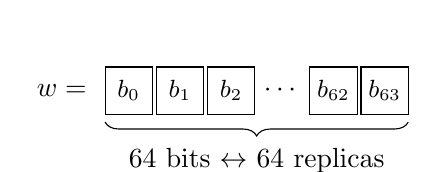
\begin{tikzpicture}
% Boîtes gauche : b_0 à b_2
\foreach \i/\label in {0/0, 1/1, 2/2} {
\draw (\i*0.65, 0) rectangle (\i*0.65+0.6, 0.6);
\node[font=\small] at (\i*0.65+0.3, 0.3) {$b_{\label}$};
}
% Points de suspension
\node at (3*0.65+0.3, 0.3) {$\cdots$};
% Boîtes droite : b_62, b_63
\foreach \i/\label in {0/62, 1/63} {
\draw (4*0.65 + \i*0.65, 0) rectangle (4*0.65 + \i*0.65+0.6, 0.6);
\node[font=\small] at (4*0.65 + \i*0.65+0.3, 0.3) {$b_{\label}$};
}
% Label gauche
\node at (-0.55, 0.3) {$w=$};
% Accolade en dessous
\draw[decorate, decoration={brace, amplitude=5pt, mirror}]
    (0, -0.1) -- (4*0.65+1*0.65+0.6, -0.1)
    node[midway, below=6pt] {64 bits $\leftrightarrow$ 64 replicas};
\end{tikzpicture}
\caption{A \texttt{Bits} $w$ encoding 64 parallel replicas. Each bit $b_i$ carries the state of replica $i$.}
\label{fig:bitword}
\end{figure}

This structure is very convenient to represent binary variable such as the spins of the system. The boolean representation $b_i \in \{0,1\}$ of a spin $s_i \in \{-1,+1\}$ is given by $b_i = (s_i+1)/2$. In that way, we are able to implement several replicas of the full spin system in a set of \texttt{Bits} $\{S_i\}$, each encoding the replicas of the associated spin, as shown in Figure~\ref{fig:spins_Bits}.

\begin{figure}[H]
\centering
\def\svgwidth{0.28\linewidth}
\input{pictures/spins_Bits.pdf_tex}
\caption{Bitwise implementation of a spin system. Each replica of the system is obtained by selecting the corresponding replica in each spin.}
\label{fig:spins_Bits}
\end{figure}



The limitation of $n_\text{bits}$ to $64$ is directly related to the architecture of modern CPUs \cite{} \noteBastien{I need some sources here}. This limit may in principle be extended up to $512$ bits
using SIMD instructions, but that requires the use of new object type in our code. This will be left for further discussion.\\



\begin{figure}[h]
\centering
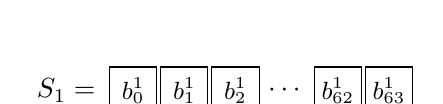
\begin{tikzpicture}
% Boîtes gauche : b_0 à b_2
\foreach \i/\label in {0/0, 1/1, 2/2} {
\draw (\i*0.65, 0) rectangle (\i*0.65+0.6, 0.6);
\node[font=\small] at (\i*0.65+0.3, 0.3) {$b_{\label}^1$};
}
% Points de suspension
\node at (3*0.65+0.3, 0.3) {$\cdots$};
% Boîtes droite : b_62, b_63
\foreach \i/\label in {0/62, 1/63} {
\draw (4*0.65 + \i*0.65, 0) rectangle (4*0.65 + \i*0.65+0.6, 0.6);
\node[font=\small] at (4*0.65 + \i*0.65+0.3, 0.3) {$b_{\label}^1$};
}
% Label gauche
\node at (-0.55, 0.3) {$S_1=$};
\label{fig:bitword}
\end{tikzpicture}
\end{figure}
\subsection{Second Optimization: Shared random numbers}
\subsection{Structure of the code}

\section{The Ising model}
\subsection{The model}
\subsection{Bitwise Implementation}
\subsection{Phase diagram}
\subsection{Performance test}
\section{The Spinglass model}
We now move on a more complex model, that is the Edwards–Anderson model.
\subsection{The Edwards–Anderson model}
The Edwards–Anderson (EA) model -- first introduced by .. \cite{SFEdwards_1975} -- is a finite dimensional spin glass model with short range interaction. It is not a mean field spin glass model with infinite range interactions such as the Sherrington–Kirkpatrick model \cite{SK_model}. The model is formally described as follows:
\begin{equation}
  H_\text{EA}=\sum_{\langle i,j \rangle}J_{ij}S_iS_j.
  \label{eq:EA_model}
\end{equation}
Where $J_{ij}$ is a random variable taking its values in $\{-1,\,1\}$ with equal probability. Thus, it can easily be represented by a \Bits.
Under a spin flip ($S_k \to - S_k$), the energy shift is:
\begin{equation}
  \Delta E_k=2 S_k \sum_{i \partial k}J_{ki}S_i.
  \label{eq:EA_energy_shift}
\end{equation}
Performing the same derivation as for the Ising model, the spin flip condition for this model is thus:
\begin{equation}
  \lfloor \rho \rfloor \geq S_k  \sum_{i \in \partial k}J_{ki}S_i,\\
  \label{eq:flip_EA_int}
\end{equation}
with $\rho$ the same exponential random variable as in the previous section.
\subsection{Bitwise Implementation}
\subsection{Performance test}

\section{The Hopfield model}
\subsection{The model}
\label{subsec:hopfield_model}
\subsection{Bitwise Implementation}
\subsection{Capacity of the Hopfield network}
\subsection{Performance test}
\include{Conclusion}
\begin{appendix}
\section*{Appendices}
\addcontentsline{toc}{section}{Appendices}

% Pour s'assurer que seules les sous-sections apparaissent dans la TOC
\addtocontents{toc}{\protect\setcounter{tocdepth}{2}}

% Redéfinition de la numérotation des sous-sections pour les appendices
\renewcommand{\thesubsection}{\Alph{subsection}}

% Appendix A
\subsection{Naive implementation of the classic Metropolis algorithm}
\begin{algorithm}[H]
\DontPrintSemicolon
\caption{Ising Metropolis sweep (classical, naive)}
\KwIn{Lattice spins $\{S_i\}$, coupling $J$, inverse temperature $\beta$}
\KwOut{Updated lattice spins $\{S_i\}$}
\BlankLine
\BlankLine
\For{$\mathrm{sweep} = 1$ \KwTo $N_{\mathrm{sweeps}}$}{
    \For{$k = 1$ \KwTo $N$}{
      \For{$r = 1$ \KwTo $n_\text{bits}$}{
          Compute $\Lambda_k = s_k^{(r)} \sum_{i \in \partial k} s_i^{(r)}$\;
          \BlankLine
          \tcp{Unconditional flip: energy is lowered}
          \eIf{$\Lambda_k^{(r)} \leq 0$}{
              $s_k^{(r)} \leftarrow -s_k^{(r)}$\;
          }{
              \tcp{Conditional flip: draw Poisson threshold}
              Draw $\lfloor \rho \rfloor$ with $\rho \sim \mathcal{E}(2\beta J)$\;
              \If{$\lfloor \rho \rfloor \geq \Lambda_k^{(r)}$}{
                  $s_k^{(r)} \leftarrow -s_k^{(r)}$\;
              }
          }
      }
    }
}
\label{alg:ising_classic_naive}
\end{algorithm}

\end{appendix}

\pagestyle{fancy}
\setlength{\bibsep}{2pt}
\bibliographystyle{unsrt}
\bibliography{references}

\end{document}
